\section{Evaluation}\label{sec-eval}

In this section we evaluate the effectiveness of Sensibility Testbed's 
privacy mechanisms, its usability as a mobile testbed, and its 
performance. To investigate whether the policies provided by 
Sensibility Testbed are representative, we surveyed the projects
in the past few years and identified their security and privacy 
mechanisms. We analyzed if Sensibility Testbed can provide policies 
to protect the corresponding data in Section~\ref{sec-our-policies}. 
We then show two examples by applying Sensibility Testbed's 
policies to two experiments in Section~\ref{sec-experiment}. We 
demonstrate that with the policies in place, we can protect the 
device owner's privacy, while the data is sufficient for answering 
research questions. We show the performance overhead of 
Sensibility Testbed in Section~\ref{sec-benchmark}, and our 
deployment experience in Section~\ref{sec-deployment}.

%\todo{Q: how well the testbed protects privacy, and still allows experiments
%to function? A: \ref{sec-accurate} and \ref{sec-function}.}


\subsection{Sensibility Testbed's Privacy Policies}\label{sec-our-policies}

\begin{table}
\scriptsize
\centering

\bgroup
\def\arraystretch{1.15}% % for table padding
\begin{tabular}{|l|l|c|c|c|}
\hline
\multirow{2}{.8cm}{\bf Project} & \multirow{2}{*}{\bf Sensor} & 
\multicolumn{3}{c|}{\bf Equivalent Sensibility Testbed policy} \\\cline{3-5}
& & {\bf Default} & {\bf Specialized} & {\bf N/A} \\\hline

EnCore~\cite{aditya2014encore}  & Bluetooth & \tickmark &   &   \\\hline
% attack: associating Bluetooth MAC address with device
% solution: use Bluetooth 4.0's native support for randomized MAC address

\multirow{2}{*}{\cite{chen2014sensor}\textsuperscript{*}} & Accelerometer 
& \tickmark &   &  \\ \cline{2-5}
& Camera & & \tickmark & \\ \hline
% attack: 2D photo/video attack (use other's photo/video as input to facial recognition) 
% and virtual camera attack (using a virtual cam to modify videos)
% solution: (1) use accelerometer to infer the orientation of front camera, 
% (2) user shaking the phone, and separate the data of shaking video and
% shaking accelerometer to ensure a real 3D face

\multirow{5}{.8cm}{ProtectMyPrivacy \cite{agarwal2013protectmyprivacy}} & Device ID & & \tickmark & \\ \cline{2-5}
& WiFi & \tickmark &   &  \\ \cline{2-5}
& Bluetooth & \tickmark &   & \\ \cline{2-5}
& Address book & & \tickmark & \\ \cline{2-5}
& Location & \tickmark &   &   \\\hline
% attack: general privacy issues
% solution: substitute anonymized data in place by crowd sourced recommendations
 
\multirow{4}{*}{CQue~\cite{parate2013leveraging}}  & Location & \tickmark &  & \\\cline{2-5}
& Accelerometer & \tickmark &   &  \\ \cline{2-5}
& Gyroscope & \tickmark &   &  \\ \cline{2-5}
& Bluetooth & \tickmark &   &   \\\hline
% attack: this paper tries to infer individual behavior by fusing a bunch of sensors 
% and provide insights into privacy leakage (use issue what-if queries to explore
% the leakage if certain sensor data is revealed to apps)
% solution: detection and fusion of sensors (math)

\multirow{3}{*}{MaskIt~\cite{gotz2012maskit}} & Location & \tickmark &   & \\\cline{2-5}
& Cellular & \tickmark &   &   \\ \cline{2-5}
& Bluetooth & \tickmark &   &   \\\hline
% attack: temperal correlations (heading towards hospital means the person will
% be at the hospital)
% solution: filter a user context stream that provably preserves privacy (a privacy 
% check deciding whether to release or suppress the current user context). privacy 
% is defined with respect to a set of sensitive contexts specified by the user
% sec 7.1 described data (location, cellular, bluetooth)

\multirow{3}{*}{Jigsaw~\cite{lu2010jigsaw}} & Accelerometer 
& \tickmark &   &  \\ \cline{2-5}  
& Microphone  & & \tickmark & \\ \cline{2-5}
& Location & \tickmark &   &   \\\hline
% attack: robustness to position change and energy drain
% solution: throttles the depth and sophistication of sensing when data is low quality

Cach{\'e}~\cite{amini2011cache} & Location & \tickmark &   &   \\\hline
% attack: location privacy
% solution: caching locaiton content in advance. retrieve content locally
% when it is needed. this is like approximate location with a zipcode/city

\cite{jiang2012isolating}\textsuperscript{*} & Cellular & \tickmark &   &   \\\hline
% attack: voice related fraud (dial a number without the user knowing it)
% solution: detect voice-related fraud activities using call records, 
% use voice calls from domestic callers to foreign recipients and 
% a Markov Clustering based method for isolating dominant fraud 
% activities from international calls

\multirow{2}{*}{TapPrints~\cite{miluzzo2012tapprints}} & Accelerometer 
& \tickmark &   &  \\ \cline{2-5}  
& Gyroscope & \tickmark &   &  \\ \hline
% attack: monitor user inputs like keyboard and icons
% solution: this is an attack paper, showing it's possible to infer location
% of taps using motion sensor + machine learning
% in Sec 4 they mentioned they had to use sensor rate@100Hz

\multirow{4}{.8cm}{FindingMiMo \cite{shin2011findingmimo}} 
& WiFi & \tickmark &   &  \\ \cline{2-5}
& Location & \tickmark &  & \\\cline{2-5}
& Accelerometer & \tickmark &   &  \\ \cline{2-5}
& Magnetometer & \tickmark &   &  \\ \hline
% attack: this is a tracker for device. it tracks and locates a missing mobile device
% in indoor environments by observing the ambient features such as radio signals, 
% and retrieving location information from ambient observations

ACCessory~\cite{owusu2012accessory} & Accelerometer & \tickmark &   
&  \\ \hline
% attack: accelerometer can be extracted to monitor inputs
% solution: this is an attack paper, showing it's possible to extract entered 
% text. in Sec 4.1/Fig 5 they mentioned sensor rate@100Hz significantly
% improved accuracy.

TouchLogger~\cite{cai2011touchlogger} & Gyroscope & \tickmark &   
&  \\ \hline
% attack: gyroscope can be extracted to monitor inputs
% solution: this is an attack paper, showing it's possible to infer 
% input using gyroscope

\multirow{6}{*}{MockDroid~\cite{beresford2011mockdroid}} 
& Location & \tickmark &  & \\\cline{2-5}
& Internet\textsuperscript{\dag} & \tickmark & & \\ \cline{2-5}
& Cellular & \tickmark &   &  \\ \cline{2-5}
& Address book & & \tickmark & \\ \cline{2-5}
& Device ID & & \tickmark & \\ \cline{2-5}
& Broadcast intent &  & \tickmark  &  \\ \hline
% attack: general privacy attacks
% solution: modify the Android OS to allow users to mock or revoke
% access to data during run time (simulating lack of location info, wireless
% network, fake device ID, never sending broadcast intent, etc.)

\multirow{6}{*}{Guardian \cite{zhang2015leave}} 
& Bluetooth & \tickmark &   & \\ \cline{2-5}
& Internet\textsuperscript{\dag} & \tickmark & & \\ \cline{2-5}
& Microphone  & & \tickmark & \\ \cline{2-5}
& Cellular & \tickmark &   &  \\ \cline{2-5}
& Motion sensors & \tickmark &   &  \\ \cline{2-5}
& CPU usage\textsuperscript{\ddag} & \tickmark & & \\\hline
% attack: rumtime information gathering (a malicious app recording
% phone conversations, etc.)
% solution: pause suspicious background apps (that records the phone 
% conversation) when the target app is running in the foreground. the 
% background apps are identified by their behaviors inferred from their
% thread names, CPU scheduling, kernel time etc. the key is when to 
% suspend and resume the suspicious background apps

\cite{aviv2012practicality}\textsuperscript{*} & Accelerometer & \tickmark &   
&  \\ \hline
% attack: accelerometer can be extracted to monitor inputs
% solution: another attack paper. their method is sample-rate independent. 
% in Tab 1 they used rates from 25 to 62Hz. on page 8, "all devices perform well
% above random guessing, suggesting that the features are reasonably
% resilient to sample rate fluctuations, as addressed by the samplenormalized
% features (see Section 6)"

\multirow{2}{*}{\cite{cai2012practicality}\textsuperscript{*}} & Accelerometer 
& \tickmark &  &  \\ \cline{2-5}
& Gyroscope & \tickmark & &  \\ \hline
% attack: accelerometer and gyroscope can be extracted to monitor inputs
% solution: another attack paper. they showed attack remains effective 
% even though the accuracy is affected by user habits, device dimension, 
% screen orientation, and keyboard layout. 

AccelPrint~\cite{dey2014accelprint} & Accelerometer & \tickmark &   
&  \\ \hline
% attack: use accelerometer to fingerprint devices
% solution: this is a fingerprinting paper. one can fingerprint an accelerometer
% when it is vibrating (eg, during an incoming call) and measure its imperfection

\multirow{8}{*}{\cite{bojinov2014mobile}\textsuperscript{*}} & Microphone  
& & \tickmark & \\ \cline{2-5}
& Accelerometer & \tickmark &   &  \\ \cline{2-5}
& Gyroscope & \tickmark & &  \\ \cline{2-5}
& Magnetometer & \tickmark &   &  \\ \cline{2-5}
& Ambient light & \tickmark &   &  \\ \cline{2-5}
& Location (GPS) & \tickmark &   &  \\ \cline{2-5}
& Touch screen & & & \xmark \\ \cline{2-5}
& Camera & & \tickmark & \\ \hline
% attack: 
% solution:

Gyrophone~\cite{michalevsky2014gyrophone} & Gyroscope 
& \tickmark & &  \\ \hline
% attack: 
% solution:

\cite{shokri2011quantifying}\textsuperscript{*}
& Location & \tickmark &   &  \\ \hline
% attack: 
% solution:

\cite{polakis2015s}\textsuperscript{*}
& Location & \tickmark &   &  \\ \hline
% attack: 
% solution:

AnonySense~\cite{kapadia2008anonysense} 
& Location & \tickmark &   &  \\ \hline
% attack: 
% solution:

\cite{liu2015good}\textsuperscript{*} 
& Accelerometer & \tickmark &   &  \\ \hline
% attack: 
% solution:

LP-Guardian~\cite{fawaz2014location} 
& Location & \tickmark &   &  \\ \hline
% attack: 
% solution:

\cite{bordenabe2014optimal}\textsuperscript{*}
& Location & \tickmark &   &  \\ \hline
% attack: 
% solution:

PrivStats~\cite{popa2011privacy}
& Location & \tickmark &   &  \\ \hline
% attack: 
% solution:

\multirow{5}{*}{ipShield~\cite{chakraborty2014ipshield}} 
& Location (GPS) & \tickmark &   &  \\ \cline{2-5}
& Accelerometer & \tickmark &   &  \\ \cline{2-5}
& Gyroscope & \tickmark & &  \\ \cline{2-5}
& WiFi & \tickmark &   &  \\ \cline{2-5}
& Cellular & \tickmark &   & \\ \hline
% attack: 
% solution:
 
\multirow{3}{*}{TaintDroid~\cite{enck2014taintdroid}} & Location & \tickmark &   &  \\ \cline{2-5}
& Accelerometer & \tickmark &   &  \\ \cline{2-5}
& Internet\textsuperscript{\dag} & \tickmark & & \\ \hline
% attack: 
% solution:

\multicolumn{5}{l}{\textsuperscript{*}\scriptsize These projects do not have a project name.} \\ 

\multicolumn{5}{l}{\textsuperscript{\dag}\scriptsize Internet connectivity policies
can be implemented by interposing socket calls.} \\

\multicolumn{5}{l}{\textsuperscript{\ddag}\scriptsize CPU usage can be obtained
through reading the files in \path{/proc/stat}.} \\

\end{tabular}
\egroup

\caption{\small Sensibility Testbed's support for privacy and security policies. A default 
policy is supported by Sensibility Testbed without extra effort. A specialized policy can 
be supported by extending default policies. A policy is marked as N/A if it is not possible 
to provide support.}
\label{tab:policy}
%\vspace{-10pt}
\end{table}

%\todo{Q1: does ST protect privacy sufficiently?}

\begin{table}
\scriptsize
\centering

\bgroup
\def\arraystretch{1.15}% % for table padding
\begin{tabular}{|l|l|c|c|c|}
\hline
\multirow{2}{.8cm}{\bf Project} & \multirow{2}{*}{\bf Sensor} & 
\multicolumn{3}{c|}{\bf Equivalent Sensibility Testbed policy} \\\cline{3-5}
& & {\bf Default} & {\bf Specialized} & {\bf N/A} \\\hline

Koi~\cite{guha2012koi} & Location & \tickmark &   &  \\ \hline
% attack: 
% solution:

Locaccino~\cite{toch2010empirical} & Location & \tickmark &   &  \\ \hline
% attack: 
% solution:

\multirow{2}{*}{Accomplice~\cite{han2012accomplice}} & Location & \tickmark &   &  \\ \cline{2-5}
& Accelerometer & \tickmark &   &  \\ \hline
% attack: 
% solution:

\multirow{2}{*}{TapLogger~\cite{xu2012taplogger}} & Gyroscope & \tickmark &   &  \\ \cline{2-5}
& Accelerometer & \tickmark &   &  \\ \hline
% attack: 
% solution:

\multirow{2}{*}{\bf Total} & \multirow{2}{*}{\bf 74} & \multirow{2}{1cm}{\bf 
63/74 (85.14\%)} & \multirow{2}{1cm}{\bf 10/74 (13.51\%)} & 
\multirow{2}{1cm}{\bf 1/74 (1.35\%)} \\ & & & & \\\hline

\end{tabular}
\egroup

\caption{\small Table~\ref{tab:policy} continued --- Sensibility Testbed's support 
for privacy and security policies. }
\label{tab:policy-continued}
%\vspace{-10pt}
\end{table}


\textbf{Privacy and security concerns.}
In order to identify the current privacy and security concerns on mobile 
devices, we surveyed 31 projects in the past few years. We then analyzed
these projects by reading their corresponding publications, identified 
their needs or their provided mechanism for privacy protection. 
These projects, listed in Table~\ref{tab:policy} and \ref{tab:policy-continued},
range from social network applications~\cite{aditya2014encore} to facial
recognition algorithms~\cite{chen2014sensor}. If their privacy need or privacy
protection can be supported by equivalent \textit{default} policies in Sensibility 
Testbed, a \tickmark\ is marked in the default column. These sensors belong to 
low to moderate risk, as defined in Table~\ref{tab:default}. Similarly, if the
sensors are of high risk, a \tickmark\ is marked in the specialized column. 
This means that a different IRB procedure could be followed to extend 
default policies (Section~\ref{sec-motivation}). If a sensor cannot be 
supported by a default or specialized policy, a \xmark\ is marked in the 
N/A column. 

Out of these projects, 
19 of them proposed privacy protection about location information, 16 of 
them considered motion sensors such as accelerometer and gyroscope 
risky, and 9 had concerns about wireless network such as WiFi and Bluetooth
(connection/pairing history, MAC addresses, etc.). As expected, location (mainly GPS)
and motion sensors (mainly accelerometer) have the most privacy and security 
concerns~\cite{chakraborty2014ipshield}.
%\todo{Q1.1: what privacy concerns do people have? }

\textbf{Are Sensibility Testbed's policies sufficient?}
As shown in Table~\ref{tab:policy} and \ref{tab:policy-continued}, nearly 86\% 
of the security and privacy issues in prior projects can be addressed in 
Sensibility Testbed using default policies, and 13\% issues can be resolved by extending 
default policies (specialized policies). Only about 1\% of them cannot
be protected by the policies in Sensibility Testbed, \yanyan{I'm not sure 
yet how to explain this. I don't know what experiment would need this.}

In particular, prior work shows 
that Android users' touch inputs can be revealed through a few attack 
techniques like keyloggers and fingerprinting. 
%For example, a smartphone's accelerometer 
%and gyroscope can disclose shift and rotation data when a user types 
%through a software keyboard. Imprecisions in sensor calibration can 
%result in a device-specific scaling and thus can be a reliable fingerprint 
%of the device. 
User generated data thus can be informative enough 
for malware to infer the key the user enters~\cite{cai2011touchlogger, 
owusu2012accessory}, or to fingerprint and identify individual 
devices~\cite{bojinov2014mobile, dey2014accelprint}. Because these 
motion sensors are accessible 
%through JavaScript in a mobile web browser, 
without requesting any 
permissions or notifying the device owner, these attack techniques are much 
less detectable. However, the chance for these techniques to succeed
depends on their sampling rate. 
%Consider an Android 
%user's average typing speed of 3 keys per second, when the sampling 
%rate goes down to once per second, the best the adversary can do is 
%just to identify 1 of these 3 keys. 
Therefore, the policies to restrict the access rates to motion sensors 
are effective when the allowed rate is lower than the best keylogger 
would require to identify a key, or the best tracker to fingerprint a device.
Section~\ref{sec-experiment} shows such an example. 

Another line of attack is on location privacy. \yanyan{need to wirte more here.
should we do an experiment for location?}

%\todo{Q1.2: does ST address these concerns? A1.2: show
%  a handful of past experiments with a 90/10 rule -- 90\% of experiments
%  can be doone with virtually no mods, and the other 8\% we can write 
%  specialized policy for and 2\% it's too hard.}

\subsection{Privacy Protection and Experiment Functionality}\label{sec-experiment}

\todo{Q2: is ST useful for answering research questions? A:
compare the results of an algorithm with varying levels of 
data precision (Seth's algorithm?), and show a diagram suggested
by Justin.}

\yanyan{with the privacy protection in place, is the data we 
provide sufficient for experiments to function?}

Research has shown that using sensors on a modern smartphone, such as 
a speaker~\cite{das2014poster}, microphone~\cite{clarkson2012breaking} 
or accelerometer~\cite{bojinov2014mobile, dey2014accelprint}, one can 
build a robust device fingerprint that is independent of the software state
and survives a hard reset. The more recent accelerometer based fingerprinting
is particular interesting because an accelerometer is accessible in mobile apps
without requesting any permissions from the device owner. Specifically, the 
technique in~\cite{bojinov2014mobile} is based on the device-specific errors in 
accelerometer calibration, which result in unique scaling and translation of 
the measured values. In this section, we show that by using data blurring in 
\sysname, it is possible to prevent such fingerprinting, while producing data that
is still sufficient for benign experiments to function. 


\begin{figure*}
\centering
\begin{subfigure}[b]{.25\textwidth}
  \centering
  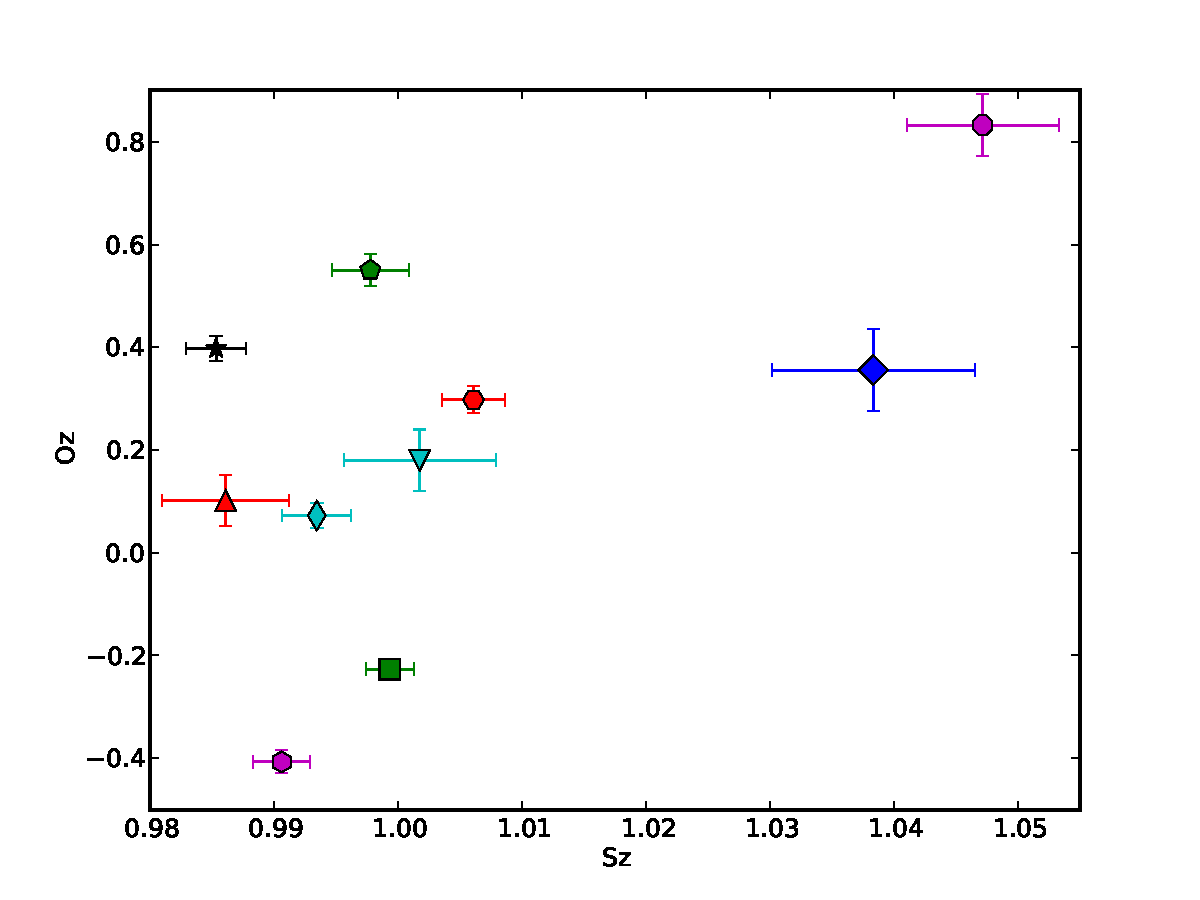
\includegraphics[width=\textwidth, trim={.9cm .5cm 1.8cm 1.3cm},clip]{figs/sz-oz.pdf}
  \caption{Data without blurring.}
  \label{fig:sub1}
\end{subfigure}%
\begin{subfigure}[b]{.25\textwidth}
  \centering
  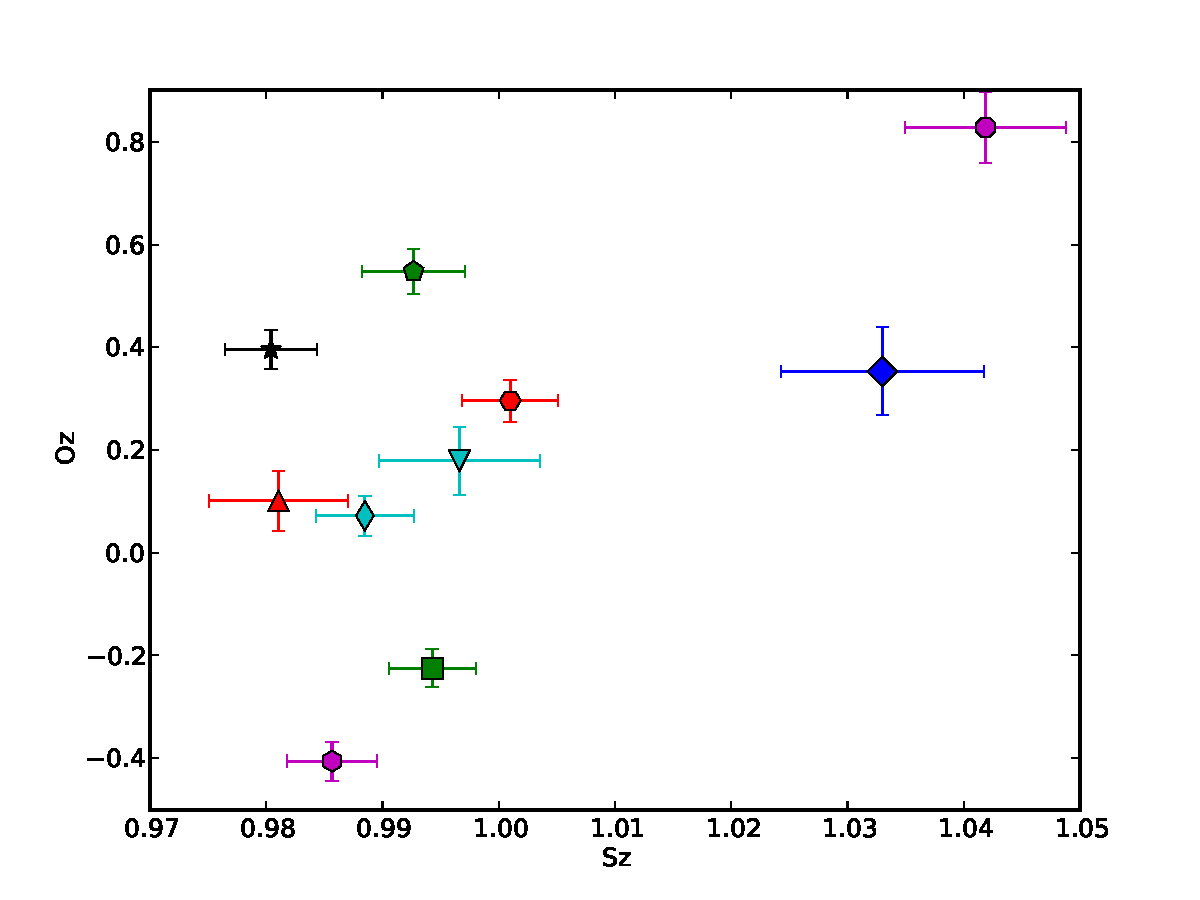
\includegraphics[width=\textwidth, trim={.9cm .5cm 1.8cm 1.3cm},clip]{figs/sz-oz-rand10.pdf}
  \caption{$[0, 10^{\circ}]$ rotation.}
  \label{fig:sub2}
\end{subfigure}%
\begin{subfigure}[b]{.25\textwidth}
  \centering
  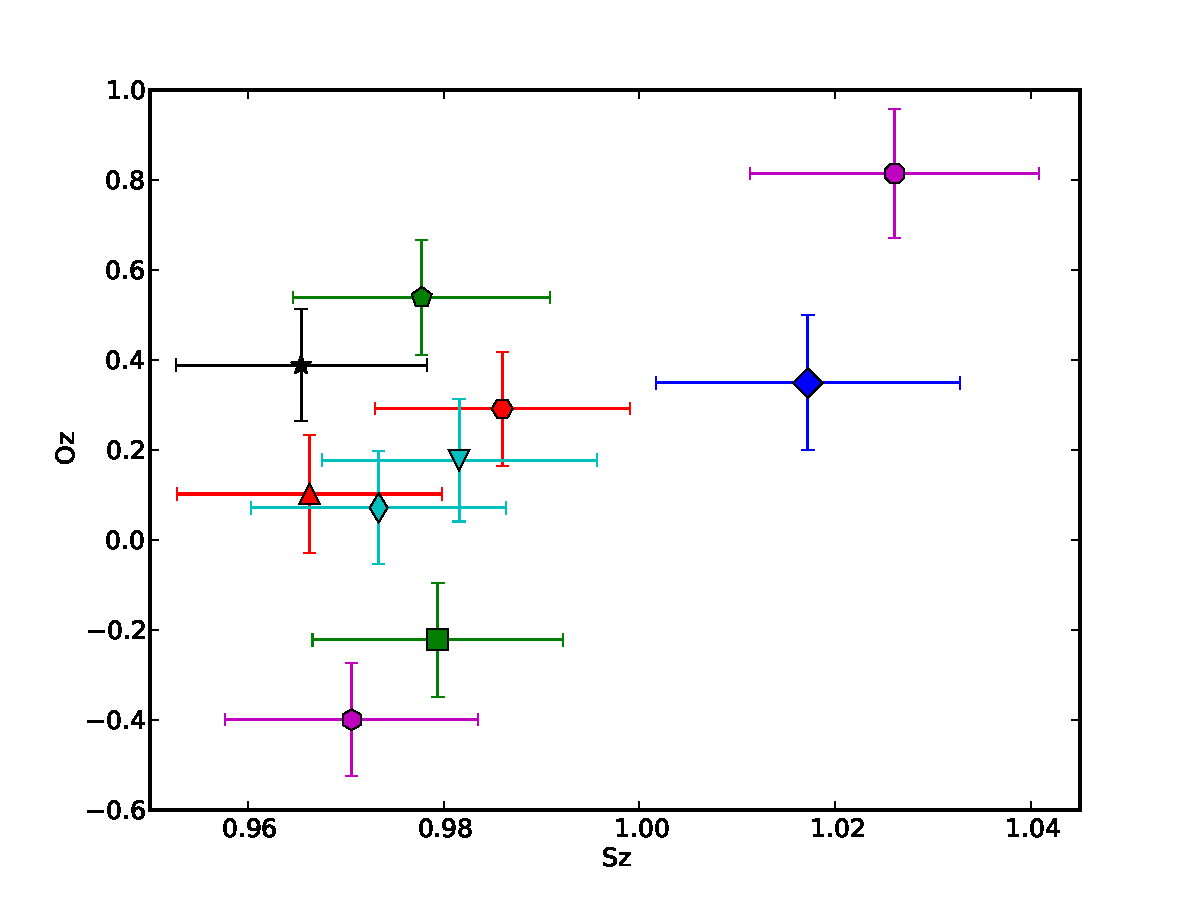
\includegraphics[width=\textwidth, trim={.9cm .5cm 1.8cm 1.3cm},clip]{figs/sz-oz-rand20.pdf}
  \caption{$[0, 20^{\circ}]$ rotation.}
  \label{fig:sub3}
\end{subfigure}%
\begin{subfigure}[b]{.25\textwidth}
  \centering
  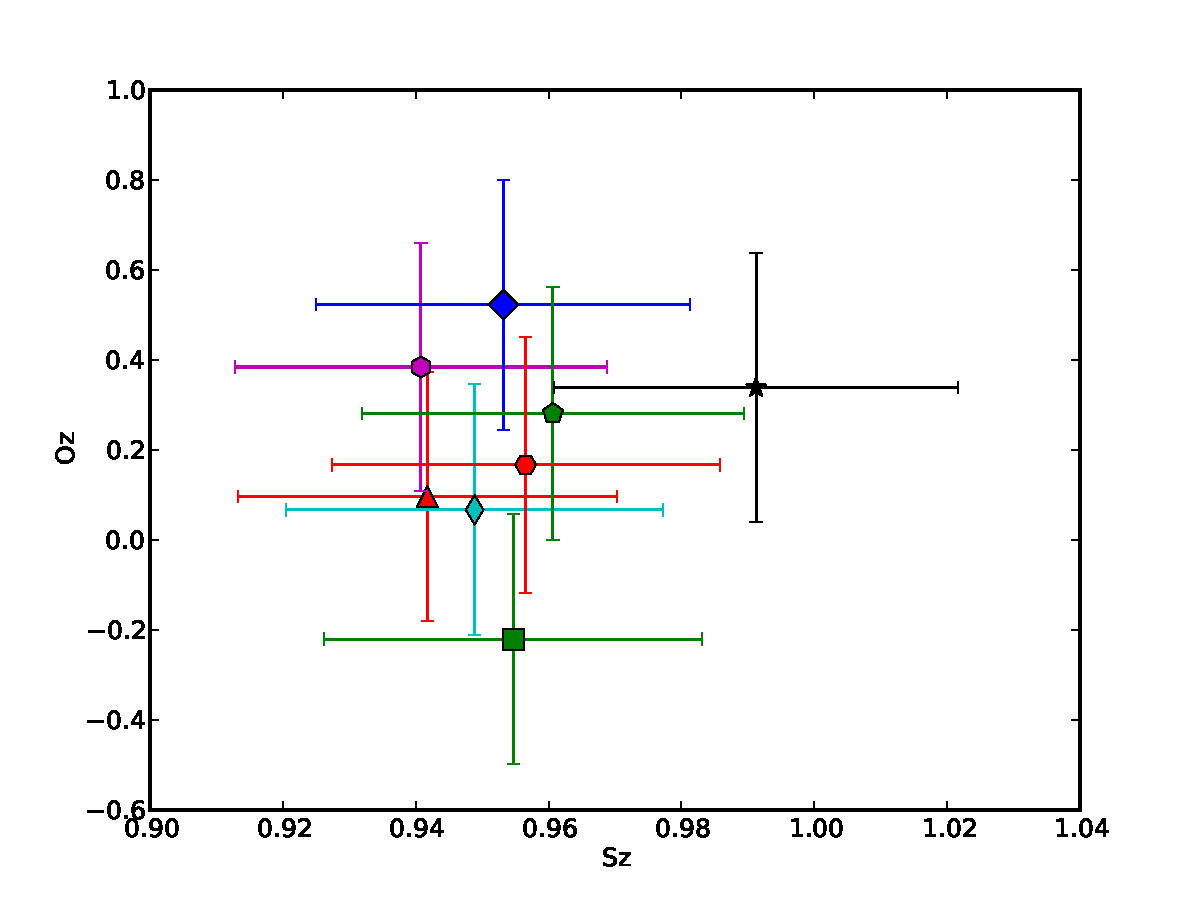
\includegraphics[width=\textwidth, trim={.9cm .5cm 1.8cm 1.3cm},clip]{figs/sz-oz-rand30.pdf}
  \caption{$[0, 30^{\circ}]$ rotation.}
  \label{fig:sub3}
\end{subfigure}%

\caption{\small Accelerometer fingerprinting without blurring, and with different levels of 
blurring that partially randomize the accelerometer data. Each device's $S_z$-$O_z$
pair is represented by the median and standard deviation of $10,000$ data samples.
\yanyan{it's better to draw a scatter plot with the result of a clustering alg overlaid on it.}}

\label{fig:fingerprinting}
\end{figure*}

\textbf{Background on accelerometer calibration.}
An accelerometer measures the acceleration force to a device along three 
physical axes. However, during the manufacturing and assmebly process, 
imperfections or variations are introduced for each individual hardware 
instance, resulting in biases in the sampled data that are unique to a specific
accelerometer~\cite{doscher1998accelerometer}. The value of a measurement
by an accelerometer, denoted by $v_m$, can be approximated as a linear 
funciton of its true value, denoted by $v_t$, as $v_m=v_tS+O$. $S$ and $O$
are the sensitivity and offset of the accelerometer, respectively. If an 
accelerometer has no calibration bias, then $S=1$ and $O=0$. Note that
this linear bias is an approximation of the real bias. In practice, $S$ and $O$
manifest randomness.

\textbf{Estimating biases along one axis.}
Like in~\cite{bojinov2014mobile}, we take advantage of the Earth's gravity
$g$, and analyze the biases along the $Z$-axis, $S_z$ and $O_z$. To 
estimate two unknows, $S_z$ and $O_z$, we need two measurements: an
accelerometer's measurement value along the $Z$-axis when the device is 
facing up ($z_m^+$) and facing down ($z_m^-$). Therefore, we have

\begin{equation}\label{eq:fxy}
\left\{
    \begin{array}{c}
      S_z = (z_m^+ - z_m^-)/2g \\
      O_z = (z_m^+ + z_m^-)/2
    \end{array}
  \right..
\end{equation}

The authors of~\cite{bojinov2014mobile} showed that this method 
produces very satisfactory results in a range of settings even 
if the surface on which the phone lies is not perfectly level.

\textbf{Data blurring and fingerprinting.}
We carried out an accelerometer fingerprinting experiment on a group
of X Android devices, with $10,000$ measurement samples from each.
Figure~\ref{fig:fingerprinting}(a) shows the estimated $S_z$ and $O_z$
based on unfiltered accelerometer data. The fingerprinting method is
very effective. Among the X devices, only one pair is near-collision. In
Figure~\ref{fig:fingerprinting}(b)-(d), we apply a blurring layer to the 
accelerometer that rotates the device by a small angle $\theta$. In 
Figure~\ref{fig:fingerprinting}(b), $\theta$ is a random variable that is
uniformly distributed between $0$ and $10^{\circ}$. Similarly, $\theta$
in Figure~\ref{fig:fingerprinting}(c) and (d) is uniformly distributed 
between $0$ and $20/30^{\circ}$. As shown, the more we rotate the 
device, the less distinct the estimation of $S_z$ and $O_z$ are for each 
device. The results in Figure~\ref{fig:fingerprinting}(c) are almost 
undistinguishable. Therefore, using data blurring in \sysname, we are able 
to prevent fingerprinting and keep the anonymity of mobile devices in such 
a case.

%\subsection{Usability}\label{sec-usability}
%
%\yanyan{user survey on privacy: show how people feel if their 
%privacy has been protected, whether device owners feel the 
%protection is enough.}
%
%\yanyan{incentives to participants}

\subsection{Microbenchmarks}\label{sec-benchmark}

We measured the overhead incurred by running blurring layers with 
experiment code in Sensibility Testbed, to demonstrate that it is 
feasible to protect sensor data privacy on end-user devices without 
affecting user experience. 
%in terms of app responsiveness and battery life.

\begin{figure}
\center{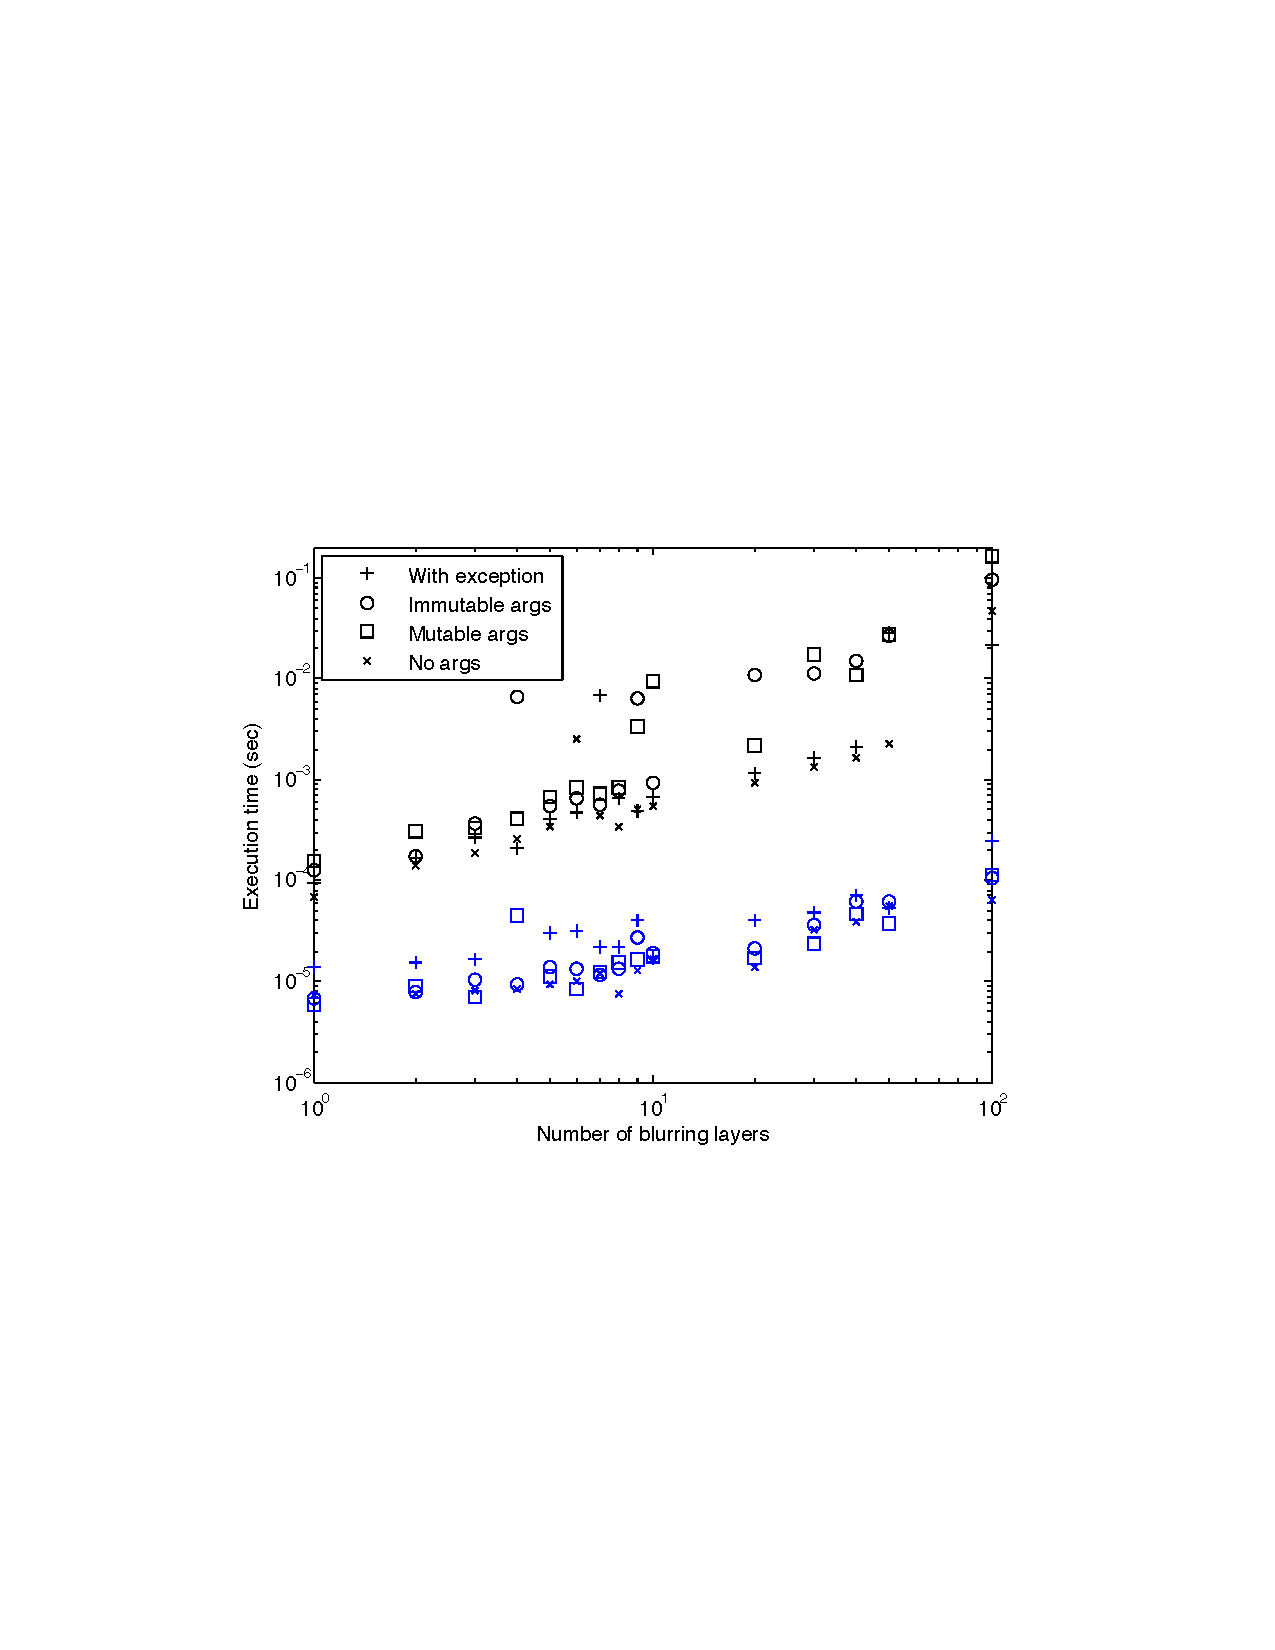
\includegraphics[width=3in]{figs/time.pdf}}
\caption{\small Overhead incurred by running varying number of blurring 
layers with experiment code. Blue points show the execution time of 
an experiment using blurring layers without verifying the runtime behavior. 
Black points show the execution time with the runtime behavior verified. 
\label{fig-time}}
\end{figure}

%\textbf{Runtime overhead.}
Figure~\ref{fig-time} shows the runtime overhead of using varying number of 
blurring layers, i.e., policies, to protect sensor data. The experiment code 
uses calls \path{get_battery()} in the Repy sandbox. Each point in the 
figure is averaged over 100 iterations. Blue points show the execution time of 
using blurring layers without verifying the runtime behavior. Black points 
show the execution time with the runtime behavior verified, i.e., using a 
contract to check arguments, return values and exceptions. Note that a 
contract checks for both mutable and immutable data types~\cite{muta} 
for arguments and return values. When the number of layers is below 10, 
the runtime is slightly increased from 10$^{-5} s$ to 10$^{-4} s$. Although
the runtime overhead is higher with more layers, as Table~\ref{tab:policy} 
and \ref{tab:policy-continued} show, most projects need less than 10
policies. 

Table~\ref{tab:overhead}(a) shows the total runtime overhead when an experiment
calls \path{get_accelerometer()}, without any blurring layer (no layer), with blurring 
layers but without verifying the runtime behavior (no-op), and with blurring layers
that verifies the runtime behavior and rounds up accelerometer to two decimal 
points (round-up). As shown in the table, the total runtime is \textit{linear} with an 
increasing number of layers/policies. The overhead per policy is almost
constant, with no-op round 0.12 - 0.14 $ms$ and round-up 0.14 - 0.21 $ms$. 
Therefore, the runtime overhead will not affect conducting an 
experiment or user experience.

Table~\ref{tab:overhead}(b) shows the memory overhead without any blurring layer 
(no layer), and with blurring layers that verifies the runtime behavior and rounds up 
decimal points (round-up). As the results show, the memory overhead is almost
constant, around 0.48 - 0.55 $MB$, until the number of blurring layers reaches 100. 
\yanyan{is there an explanation?} Nevertheless, the overhead never exceeded 1 
$MB$ in all cases. 

\begin{table}
\scriptsize
\centering

\bgroup
\def\arraystretch{1.15}% % for table padding

\begin{tabular}{|l|l|c|c|c|c|}
\hline
\multicolumn{2}{|c|}{\multirow{2}{*}{\bf Operations}} & 
\multicolumn{4}{c|}{\bf Number of blurring layers} \\\cline{3-6}
\multicolumn{2}{|c|}{} & {\bf 3} & {\bf 10} & {\bf 50} & {\bf 100}\\\hline

\multicolumn{2}{|c|}{No layer (baseline)} & \multicolumn{4}{c|}{6.276 $ms$} \\\hline

\multirow{2}{*}{No-op} & Total & 6.654 $ms$ & 7.756 $ms$ & 12.75 $ms$ & 18.94 $ms$ \\ 
& Per-layer & 0.1259 $ms$ & 0.1479 $ms$ & 0.1295 $ms$ & 0.1266 $ms$ \\\hline

\multirow{2}{*}{Round-up} & Total & 6.907 $ms$ & 7.991 $ms$  & 13.86 $ms$ & 20.64 $ms$ \\ 
& Per-layer & 0.2104 $ms$ & 0.1715 $ms$ & 0.1518 $ms$ & 0.1436 $ms$ \\\hline 
\multicolumn{6}{c}{\vspace{-0.1cm}}\\

\multicolumn{6}{c}{\small (a) Runtime overhead.} \\
\end{tabular}\\\vspace{0.25cm}
%\end{subtable}


\begin{tabular}{|l|l|c|c|c|c|}
\hline
\multicolumn{2}{|c|}{\multirow{2}{*}{\bf Operations}} & 
\multicolumn{4}{c|}{\bf Number of blurring layers} \\\cline{3-6}
\multicolumn{2}{|c|}{} & {\bf 3} & {\bf 10} & {\bf 50} & {\bf 100}\\\hline

\multicolumn{2}{|c|}{No layer (baseline)} & \multicolumn{4}{c|}{6.246 $MB$} \\\hline

\multicolumn{2}{|c|}{Round-up} & 6.742 $MB$ & 6.801 $MB$ & 6.727 $MB$ & 7.230 $MB$ \\\hline

\multicolumn{2}{|c|}{Overhead} & 0.492 $MB$ & 0.555 $MB$ & 0.480 $MB$ & 0.984 $MB$ \\\hline
\multicolumn{6}{c}{\vspace{-0.1cm}}\\

\multicolumn{6}{c}{\small (b) Memory overhead.} \\
\end{tabular}
%\end{subtable}

\egroup

\caption{\small Overhead with varying number of blurring layers. }
\label{tab:overhead}
%\vspace{-10pt}
\end{table}


%\textbf{CPU and memory overhead.}
%\todo{what's the CPU/memory overhead?}

\subsection{Deployment Experience}\label{sec-deployment}

%\todo{Q3: how is the testbed being used? A: deployment experience: 
%number of people, projects, issues, hackathon.}

%\subsubsection{External Projects and Collaboration}\label{sec-external}

Sensibility Testbed has been adopted by projects such as 
Open3G~\cite{open3g} that investigates on cellular technologies 
and coverage, a vehicle data collection project~\cite{reininger2015first} 
that monitors vehicle traffic patterns. The experience from the 
project developers was positive, and they identified cases where our 
instructions for use were unclear. Despite these clarification issues, in 
the case of Open3G, the developer reported that writing the code to
get cellular information took about an hour and they have used our
testbed since 2012. We are currently in discussions with other 
researchers about integrating Sensibility Testbed into their research
projects, such as monitoring construction safety.

In 2014, we hosted a Hack-a-thon styled, one-day workshop co-located with 
the IEEE Sensors Applications Symposium (SAS) \cite{sas}. About twenty 
workshop participants with various backgrounds worked in teams 
for six hours and built four functional applications using Sensibility 
Testbed. None of the participants had any prior experience with 
this testbed, and many of them had no background in Computer
Science. With this success, we hosted a second workshop with 
SAS in 2015, and will continue in 2016. Interesting experiments 
developed by the participants include a device network monitor: 
when the battery level of a device is low, WiFi or Bluetooth that 
requires high power is turned off.

\textbf{Ease of use.}
%\label{sec-ease}
\todo{Q4: how easy is it to use the testbed? A: ease of use: 
compared to common measurement app (Android), 
how many lines of code can one save.}

\yanyan{how much time a student spent doing some
measurements (like Thomas's motion detection alg).}

\yanyan{compare to other projects,  developers can save
thousands of lines of code, and reuse the same set of 
devices.}
